

\documentclass[runningheads]{llncs}

\usepackage[hyphens]{url}
\usepackage{hyperref}
\usepackage{graphicx}
\usepackage{afterpage}
\usepackage{caption}

\usepackage{subcaption}
\usepackage{float}

\title{Pristine Sentence Translation: A New Approach to a Timeless Problem}

\author{
	Meenu Ahluwalia, Brian Coari, and Ben Brock
}

\institute{Master of Science in Data Science \\ Southern Methodist University \\ Dallas, Texas USA \\
	\email{\{mahluwalia, bcoari, bbrock\}@smu.edu}}


\begin{document}
	\emergencystretch 3em
	\maketitle
	
	\begin{abstract}

In this paper, we present Pristine Sentence Translation (PST), a novel approach to language translation based upon sentence-level granularity. Traditional translation approaches, including those utilizing advanced machine learning or neural network-based approaches, translate on a word-by-word or phrase-by-phrase basis; thereby, potentially missing the context or meaning of the complete sentence. Instead of these piecewise translations, PST utilizes deep learning and predictive modeling techniques to translate complete sentences from their source language into their target language. With these approaches we were able to translate sentences that closely conveyed the meaning of the original sentences. Our results demonstrated that PST's method of translating an entire sentence is a robust approach to translations in some circumstances.
		
	\end{abstract}
	
	%\begin{keywords}
	%Data Science, Predictive Analytics, NLP, Translation, Google Cloud
	%\end{keywords}
	
	\section{Introduction}
	
	There is not a robust way to translate sentences containing colloquialisms, idioms, and other forms of slang correctly into other languages. The ability to communicate with people in another language presents a number of technical challenges. Technology has come a long way from the discovery of the Rosetta Stone in 1799, which allowed us to translate Egyptian hieroglyphics to ancient Greek in 23 years. In the modern day, tools such as Google Translate can be used in real time to convert between languages and allow people to communicate from different cultures~\cite{ref_url6}. The latest iterations of Google Translate even use machine learning and neural networks to parse word combinations instead of just single words, delivering a more satisfying user experience~\cite{ref_url7}.
	
	With the magnitudes of advancements in language translations, however, there are still areas for improvement. While Google Translate works very well with basic translations such as finding a bathroom and ordering off a menu off a menu, the intricacies and complexities of a normal, native conversation still can cause a non-fluent speaker difficulty. For example: an American coworker might mention to a Brazilian coworker about performance on a project with ``You hit one out of the park''. This is a term borrowed from the American sport of baseball, in which hitting a ball out of the ballpark is a great thing to do. The Brazilian coworker might use a traditional translation tool and get a word-for-word result of ``Você bateu um fora do parque'', but without the context of knowing about American baseball the meaning of this phrase might be lost. This situation is even greater when encountered in print, which complicates the situation because you cannot ask a book to clarify what it means.
	
	In this paper, we present Pristine Sentence Translation (PST), a novel approach to language translation based upon sentence-level granularity. This approach allows a translator to use any number of words in order to properly communicate an idea behind a sentence instead of translating the sentence word-for-word. To implement the PST solution we stored entire sentences in a database, and mapped them to entire sentences in other languages that represent the meaning of those sentences. For example: using the example above we would have an entry for the English sentence ``You hit one out of the park'', and we would have an entry for a Portuguese sentence mapped to that English sentence that says ``Você foi ótima'' which translates in English to the meaning behind the phrase: ``You did great''. 


	\begin{minipage}{\linewidth}
		\begin{center}
			\hspace*{-.5in}
			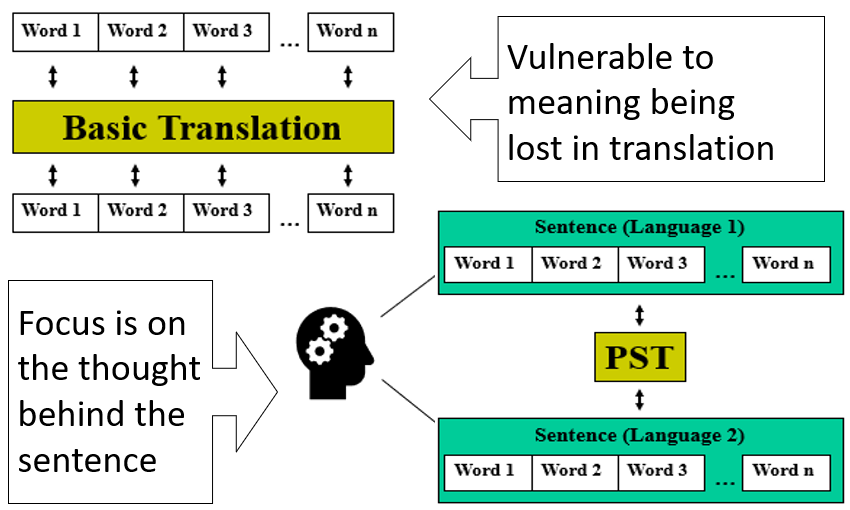
\includegraphics[width=\textwidth]{Pristine_Sentence_Translation_Visual.png}
			\captionof{figure}{Pristine Sentence Translation High-Level Overview}
			\label{fig:Pristine Sentence Translation High-Level Overview}
			\vspace*{1cm}
		\end{center}
	\end{minipage}
	\afterpage{\clearpage}

	One main issue with doing sentence-to-sentence translations is that if we do not have an exact match for the sentence, PST returns nothing. If we tried to translate ``You really hit one out of the park'' from English into Portuguese we would not get any results if all we had a translation for was ``You hit one out of the park''. We addressed this concern by removing special characters and making all input lowercase to filter out the noise in a sentence, and then used Predictive Modeling in order to find the sentence most like the input sentence, using a closeness metric of Euclidean Distance. Using this method, ``You really hit one out of the park'' would map most closely to ``You hit one out of the park'', and return the same translation: ``Você foi ótima''. We built a graphical user interface (GUI) to inform the user that the translation is not for the original input sentence, instead it indicates that it is showing results for: ``You hit one out of the park''. The algorithm also provides a percentage for how close the match was, so the user can determine if the match was close enough to be useful.
	
	Our initial version of PST focuses on translations between English, Portuguese, and German. Our input was a few hundred phrases taken from popular travel websites in order to get a good sampling of what might be needed to navigate as a foreigner in a country. We tested these sentences in order to demonstrate the effectiveness of this technique, and in this paper we display our results for review. 

	In order to find a close match between sentences for PST we needed to find a way to determine the closeness of sentences to each other. We analyzed two  methods of determining how close one sentence is to another, Euclidean Distance and Cosine Similarity, and choose the best method based on the metrics it provides for closeness. After we determine the closest match of an input sentence to one we know through our PST database, we can return a curated translation that matches that sentence in the requested language.

	By returning a curated translation to a sentence that is determined to be close to the sentence that is input we remove the granularity of a word-to-word translation, getting us closer to conveying the thoughts behind the sentence the speaker is trying to communicate. Our input data of a few hundred phrases is not sufficient to provide a close match to sentences from normal conversations, but our examples show the basic functionality of PST. With more seed data curated by language and cultural experts, PST's usefulness can grow to applications in movie or television script translation, technical documentation translation, and other forms of translation where specialized language 
	
	\section{Related Work}
	The concept of translating one language to another is one of the most prevalent topics in data science, existing tools and methods were readily available. This first tool we looked at is one of the strongest and most popular forces in translation today: Google Translate. In 2016 Google started using Deep Learning  to perform translations and saw vast reduction in errors ~\cite{ref_url18}. Even though this method was vastly superior to Google's previous system it is still dependent on the individual words in a sentence, and still subject to the same issues stated above with translations, since it would not handle colloquialisms or words that have no direct equivalent in the destination language. 

	The author developed a Neural Machine Translation System using Keras, and used a ``closeness of match'' system to translate between one language and another ~\cite{ref_url16}. This approach is much close to the spirit of PST, with the exception of only returning one sentence in the intended language. We would like an approach that allows us to find more than one sentence ID from the destination language. PST uses a similar approach, but aims to find a matching sentence ID for the input sentence, then look up all sentences that are translations for that sentence in the requested language. More details on this are provided in the ``Solution Approach'' section.
	
	\section{NLP and Neural Networks}
	The recent advances of machine learning and growing amounts of available data have made a great impact on the field of  Natural Language Processing (NLP). They facilitated development of new neural architectures and led to strong improvements on many NLP tasks, such as machine translation or text classification. 
	
	Automatic or machine translation is a challenging AI task, given the fluidity of human language. Classically, rule-based systems were used for this task, which were replaced in the 1990s with statistical methods. More recently, deep neural network models achieve state-of-the-art results in a field that is aptly named neural machine translation~\cite{ref_url16}.
	One advancement of particular importance is the development of models which build good quality, machine-readable representations of word meanings. These representations, often referred to as word embeddings, are vectors which can be used as features in neural models that process text data.
	
	Sequence to Sequence (often abbreviated to Seq2Seq) models are a special class of Recurrent Neural Network architectures typically used (but not restricted) to solve complex Language related problems like Machine Translation, Question Answering, creating Chat-bots, Text Summarization, etc. Our aim is to translate given sentence from one language to another. We target sentence translations to and from English, Portuguese and German languages. Use of Seq2Seq (or Encoder-Decoder) architecture is appropriate in this case as the length of the input sequence  does not has the same length as the output data.
	
	To summarize our Encoder-Decoder model, the Encoder simply takes the input data, and train on it then it passes the last state of its recurrent layer as an initial state to the first recurrent layer of the decoder part. The Decoder takes the last state of encoder’s last recurrent layer and uses it as an initial state to its first recurrent layer, the input of the decoder is the sequences that we want to get. We use the Keras API with Tensorflow backend to build our model.
	
	One of the important tasks for language understanding and information retrieval~\cite{ref_url26} is to model semantic similarity between words, phrases or sentences. Siamese LSTM networks seem to perform well on similarity tasks and have been used for tasks like sentence semantic similarity, recognizing forged signatures and many more.
	Siamese LSTM is a supervised learning model where input is pairs of sentences having different sequence length and a label for the pair which describe the underlying similarity between sentence pairs~\cite{ref_url21}. We use this similarity score to find the closest matched sentence from our dataset for the sentence input by the user for translation.
	
	
	\section{Approach}
	Our approach to solving the issues around language translations takes five main steps. Each step is discrete and can be run and unit-tested independently. The ``Full Demo'' section goes over what the steps look like and how they relate to each other in a full iteration of the program. 
	
	First, we form a pristine database of known, correct, contextual translations to sentences that focus on translating the intent of sentences rather than the word in that sentence. There is more detail on this step in the ``Data Collection'' section. 
	
	Second, we take input from a user on the requested translation and the languages involved in the translation. This is covered in more detail in the ``Full Demo'' section. 
	
	Third, we  implement a Sequence to Sequence model for our translations. We also develop a Siamese LSTM model to find as close a match as possible to the input sentence and its associated translation.  More details of that can be found in the  ``Encoder-Decoder Long Short-Term Memory (LSTM) Networks''  and ``Siamese LSTM for Learning Sentence Similarity'' section. 
	
	Fourth, we measure the closeness of our guessed sentence to our input sentence using Euclidean Distance and Cosine Similarity, then return the result of the method that we determine is the best performing indicator, along with all sentences that relate to the matched sentence to the front end. This is covered in more detail in the ``Euclidean Distance and Cosine Similarity'' and ``Results and Analysis'' sections.
	
	Fifth and last, we display our results to the user through the front end. This is covered in more detail in the ``Full Demo'' section.


	\begin{minipage}{\linewidth}
		\begin{center}
			\hspace*{-.3in}
			\hspace*{-.3in}
			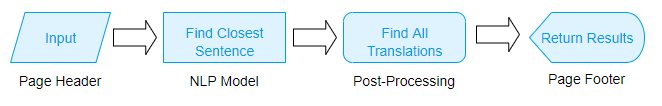
\includegraphics[width=\textwidth]{Process_Map.png}
			\captionof{figure}{Process Map}
			\label{fig:Process Map}
			\vspace*{1cm}
		\end{center}
	\end{minipage}
	\afterpage{\clearpage}
	

	
	We first collected 200 sample sentences from various travel sites in order to build a base of useful translations. Next, we developed a back end of a Google Cloud-hosted MySQL database that holds the the translations for all of our sentences and the translation relationships between those sentences. We then developed an HTML front end that allows users to request a translation of a sentence from one language to another. Once a sentence translation has been requested we used a combination of NLP and similarity metrics in order to find a close sentence match in the source language. Then we used our MySQL database to find all of the related matches to the closest-matched sentence in the language requested by the user and returned them to the UI for display, along with the percentage of how close the match was. 

	\section{Data}
	The data for this project was collected to help people who travel for business or pleasure.  While travel is becoming more accessible (with an increasing number of both travelers and destinations), the tourist may face a few communication issues when conversing with waiter, taxi driver, hotel staff etc., because of the number of different languages and countries involved. The initial collection of 200 English Sentences are those various travel sites found were valuable to know when travelling. The sentences were assembled in English from three travel websites.~\cite{ref_url11,ref_url12,ref_url13} and translated to Portuguese and German using Google Translate~\cite{ref_url14}. The translations were verified manually by a human who is proficient in Portuguese and another one in German. If the translation done by Google did not make sense, the translation was modified to make it more sensible. The list of sentences and translations can be found in our public GitHub Repository in the Appendix.
	
	Before we start building the model, we need to clean up the text data (i.e. the sentences). We removed all punctuation characters. We then normalized the case to lowercase, normalized all Unicode characters to ASCII and removed any tokens that are not alphabetic. 
\newline

	\begin{minipage}{\linewidth}
		\begin{center}
			\hspace*{-.3in}
			\hspace*{-.3in}
			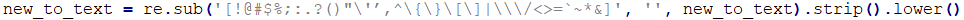
\includegraphics[width=\textwidth]{Text_Cleanup.png}
			\captionof{figure}{Text Cleanup Code}
			\label{fig:Text Cleanup Code}
			\vspace*{1cm}
		\end{center}
	\end{minipage}
	\afterpage{\clearpage}

To build the model, we needed to map words to integers  using the Keras Tokenize class. The Tokenizer had to be constructed and then fit on either raw text documents or integer-encoded text documents
	
	We also computed the vocabulary sizes and the lengths of maximum sequence for both the languages. We needed to encode each input and output sentence to integers and pad them to the maximum phrase length to make all sentences of the same length. 
	
	\subsection{Database Design}
	For our database design we leveraged a cloud-based storage system so that we could both reference the same live database around the world, as well as making the database updateable in real-time. Realtime updates allows to users to teach the program new translations for sentences for which it does not yet have a translation. We chose Google Cloud Platform (GCP) as a host for our database due to its ease of setup and robust set of no-cost features. We created a MySQL database on Cloud SQL to store our translation tables.
	
	In order to build a database that allows us to translate whole sentences easily from one language to another we needed a way to store the text of the sentences as well as the relationships between them. Our Cloud SQL MySQL database consists of two tables:
			
		\begin{enumerate}
			\item Sentences: Stores a unique Sentence ID for a combination of text (max 500 characters) and a language key (EN=English, PT=Portuguese, DE=German). There is also a place for a suggested replacement for possible future enhancements, but this is not used in our current version of the program.
			\item Translations: A table that stores the Sentence IDs that are translations of each other, linking the sentences together. These Sentence IDs are foreign keys that link to Sentence IDs in the Sentence table
		\end{enumerate}

	The use of the Translations lookup table allows us to associate any number of sentences to each other, so we can have more than one translation for a sentence, and we can maintain translations to sentences only that match up together. In the future we might have sentences in English that only have translations in German, but not Portuguese, for example. 	
\newline
	\begin{minipage}{\linewidth}
			\hspace*{-.25in}
  			 \noindent\makebox[\textwidth]{%
			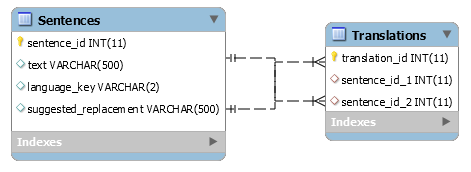
\includegraphics[width=1\textwidth]{Database_Diagram.png}}
			\captionof{figure}{Data Example}
			\label{fig:Database Diagrams}
			\vspace*{1cm}
	\end{minipage}
	\afterpage{\clearpage}

	In order to facilitate rapid and stable testing and a responsive user interface we extracted the data in the database into dataframes through sqlalchemy~\cite{ref_url15} and exported the data to .pkl files. We then loaded the .pkl files whenever we need the data for a model, which makes us immune to network interruptions and allows us faster access to our data. Examples of the SQL Queries used to extract the data can be found in Appendix A.
	

	\subsection{Euclidean Distance and Cosine Similarity}	
	For our comparison on closeness of strings we leveraged two methods: Euclidean Distance and Cosine Similarity. Euclidean Distance measures the distance between two points in a space, and therefore the minimum distance is the closest match. Cosine Similarity is the similarity between two vectors in a space, and therefore the maximum similarity is the closest match. In this section we describe how these methods calculate their scores, and in the ``Results'' section we show the result of the comparison and choose our preferred match.
	
Euclidean distance, also known as L2 distance or the Pythagorean metric, is a basic measure of distance in a space. Given a number of dimensions in a space, the Euclidean Distance calculates the length of a line segment connecting those points. This distance is calculated by going through all of the dimensions, adding up the square of the difference between the points of each value for that dimension, then taking the square root of that sum. This method is called the Pythagorean Formula.~\cite{ref_url19}. Euclidean distance is simple, but sometimes struggles if the data are not of similar shapes, as is the case with our sentence sample~\cite{ref_url19}.

Cosine Similarity tries to measure similarity in a fundamentally different way from Euclidean Distance. Instead of stepping through and comparing data point-by-point, Cosine Similarity steps through each sample and tries to build a directional vector for the shape of the data, then measures the cosine of the angle between the two vectors. In the case of text analysis, the cosine similarity uses the frequency of words in a sentence to determine a directional vector. Cosine Similarity ignores the words that are not in common between two sentences, and focuses only on words that are common, which avoids penalizing sentences that are very long and focuses on finding the most commonality. Therefore, cosine similarity is very resilient to data that is of different shapes, since the shape of the data would not necessarily affect the direction of the vector. The sentences with the closest ratios of like words would be considered a match.~\cite{ref_book1} This resilience to differently-shaped data is promising for our purposes, and seems to be a good fit for comparing sentences, and we see in the ``Results'' section that we did get results that are visually close to the requests.

	\subsection{Encoder-Decoder Long Short-Term Memory (LSTM) Networks}
	The encoder-decoder model also known as Seq2Seq model provides a pattern for using recurrent neural networks to address challenging sequence-to-sequence prediction problems, such as machine translation.
	Key to the encoder-decoder architecture is the ability of the model to encode the source text into an internal fixed-length representation called the context vector. Once encoded, different decoding systems could be used to translate the context into different languages.

	\begin{minipage}{\linewidth}
		\begin{center}
			\hspace*{-.25in}
  			 \noindent\makebox[\textwidth]{%
			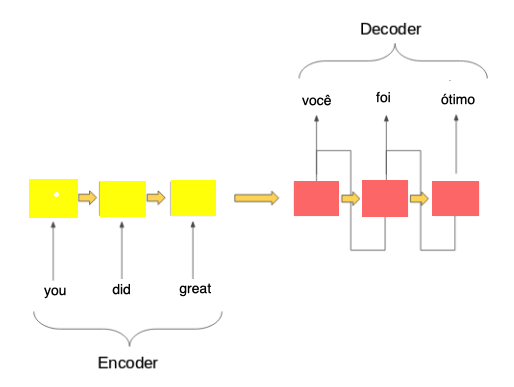
\includegraphics[width=.9\textwidth]{enc_dec_2.png}}
			\captionof{figure}{Sequence to Sequence Model}
			\label{fig:Sequence to Sequence Model}
		\end{center}
	\end{minipage}
	\afterpage{\clearpage}
	
	Our Seq2Seq model is defined as the following:
	
	\begin{enumerate}
		\item For the encoder, we used an embedding layer and an LSTM layer
		\item For the decoder, we used another LSTM layer followed by a dense layer
	\end{enumerate}
	
	\begin{minipage}{\linewidth}
		\begin{center}
			\hspace*{-.4in}
  			 \noindent\makebox[\textwidth]{%
			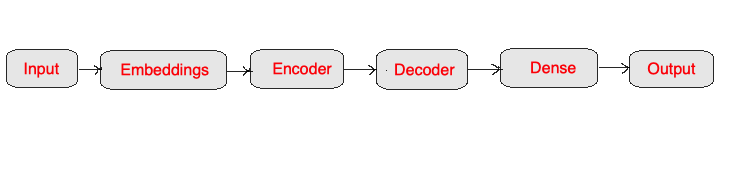
\includegraphics[width=.9\textwidth]{Seq2Seq.png}}
			\captionof{figure}{Model Architechture}
			\label{fig:Model Architectture}
		\end{center}
	\end{minipage}
	\afterpage{\clearpage}
	
	\subsubsection{Training the Neural Translation Model}
	\paragraph
	We used the English-Portuguese and  English-German sentence pairs dataset  from Anki~\cite{ref_url4}  to train our Seq2Seq model.
	The model was trained for 30 epochs and a batch size of 512 on a training set of 40,000 sentences and a hold-out set of 10,000 sentences.   
		
	As shown in Fig 7, the validation loss stopped decreasing after 20 epochs and the accuracy of the model did not improve after 20 epochs.
	
	\begin{figure}[H]
		\begin{subfigure}[b]{0.49\textwidth}
			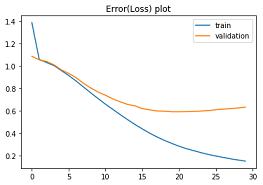
\includegraphics[width=\textwidth]{Por-Eng-Train_Loss.png}
			\label{fig:f1}
		\end{subfigure}
		\hfill
		\begin{subfigure}[b]{0.49\textwidth}
			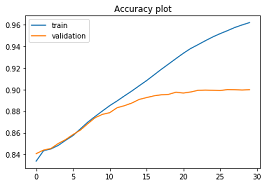
\includegraphics[width=\textwidth]{Por-Eng-Train_Acc.png}
			\label{fig:f2}
		\end{subfigure}
		\caption{Loss and Accuracy plots for Training and Validation data for Encoder-Decoder Model}
	\end{figure}
	\afterpage{\clearpage}

	Here is an excerpt of the result for finding various English sentence matches.
	
	\begin{table} 
		\begin{center}
			\begin{tabular}{| l | l | l | |}			
				\hline
				 & Actual \ & Predicted  \\
				 \hline
					1 & i have lost my passport & i lost my passport \\
				    \hline				
					2 & someone stole my money & someone stole my money \\
					\hline
					3 & i would like to order & i like to ask \\
					\hline
					4 & may i see a menu & can i see a menu \\
					\hline
					5 & i would like a drink & i want a drink   \\
					\hline
					6 & how do i call down to the front desk & how do i call to machine    \\
					\hline
				    7 & how many beds are in the room & how many are  in  room       \\
				    \hline
					8 & i dont understand & i dont understand   \\
					\hline
					9 & how are you &  how are you  \\
					\hline
					10 & how is it going & how are things    \\
				\hline
			\end{tabular}
		\end{center}
		\captionof{table}{English Sentence Matches}
		\label{table:English Sentence Matches}
	\end{table}

	The Seq2Seq English sentence matches give us an opportunity to see how well PST sentence matching works. There are several instances where it misses out on understanding the keywords. For example, when the expected translation was “i would like to order”, it translated to “i like to ask”. Although most of the translations, are visually and meaningfully close to the input, this model does not allow for more than one possible meaning of a sentence. We have been able to achieve this behavior by implementing a Siamese Network model that will be described in the next section.
	
	
	\subsection{Siamese MaLSTM for Learning Sentence Similarity}	
	Siamese networks are networks that have two or more identical sub-networks in them.
	Siamese networks seem to perform well on similarity tasks and have been used for tasks like sentence semantic similarity, recognizing forged signatures and many more
	
	In the model, there are two identical LSTM network. LSTM is passed vector representations of sentences and output a hidden state encoding semantic meaning of the sentences. Subsequently, these hidden states are compared using some similarity mechanism to output a similarity score.
	Its architecture is depicted in figure below:
	
	\begin{minipage}{\linewidth}
		\begin{center}
			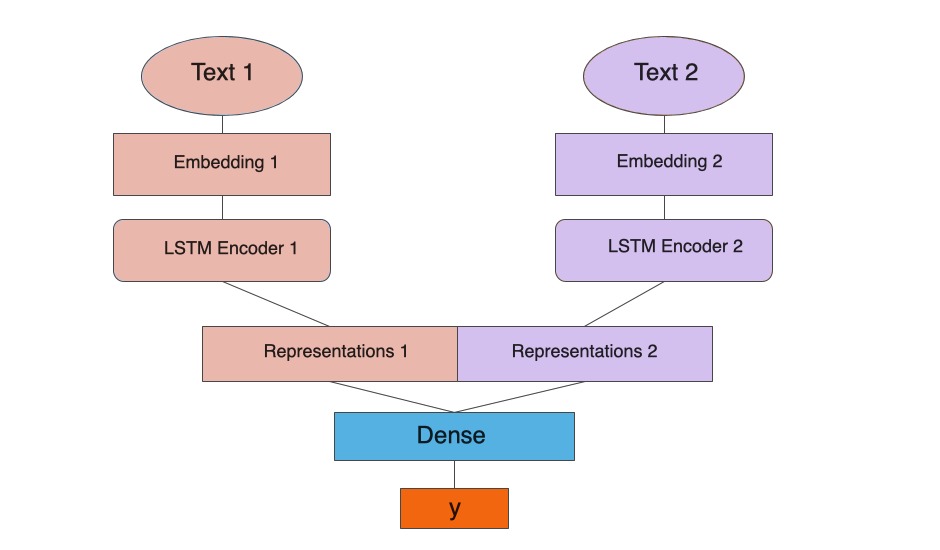
\includegraphics[width=\linewidth]{Siamese_Network.png}
			\captionof{figure}{Siamese LSTM Architechture}
			\label{fig:Siamese LSTM Architectture}
		\end{center}
	\end{minipage}
	\afterpage{\clearpage}
	
	We have two embedded matrices that represent a candidate of two similar questions.  We feed them into the LSTM (practically, there is only one) and the final state of the LSTM for each question is a 50-dimensional vector. It is trained to capture the semantic meaning of the question. By now we have the two vectors that hold the semantic meaning of each question. We put them through the defined similarity function (below):
\newline

	\begin{minipage}{\linewidth}
		\begin{center}
			\centering{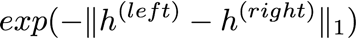
\includegraphics[width=5cm,height=4cm,keepaspectratio]{ma_similarity.png}}
			\captionof{figure}{Siamese Similarity Function}
		\end{center}
	\end{minipage}
	\afterpage{\clearpage}


	Since we have an exponent of a negative, the output (the prediction in our case) is between 0 and 1.
	
	We trained the Siamese LSTM model using Kaggle's Quora Pairs dataset~\cite{ref_url25}. 	
	
	Fig.10 shows a plot of Model Loss (MSE) and Accuracy on y-axis as a function of number of epochs on the x-axis.
	The mean squared error (MSE) is the same as loss measure of the model. The best value of training MSE obtained is 0.1179 and it is found to be decreasing at a decreasing rate throughout the training process of the model. Whereas the validation MSE is found to be 0.1257 at the end of 30 epochs.
	
	Validation accuracy which indicates the performance of model on unlabeled data is found to be 82.80\% at the end of 20 epoch after which the model does not perform as well as evident from the accuracy plot in Fig.10.
	
	\begin{figure}[H]
		\begin{subfigure}[b]{0.51\textwidth}
			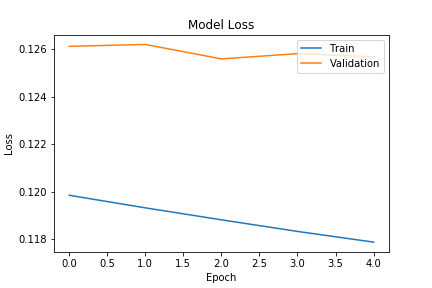
\includegraphics[width=\textwidth]{siamese_eng_loss.png}
			\label{fig:Model Loss}
		\end{subfigure}
		\hfill
		\begin{subfigure}[b]{0.51\textwidth}
			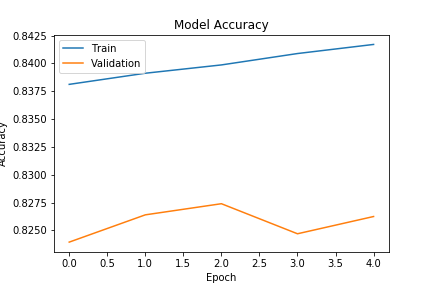
\includegraphics[width=\textwidth]{siamese_eng_acc.png}
			\label{fig:Model Accuracy}
		\end{subfigure}
		\caption{Loss and Accuracy plots for Training and Validation data for Siamese Network}
	\end{figure}
	
	The test dataset consists of 200 sentences that were collected from travel sites as stated in the Data Collection section above. The sentence input by the user is compared with every sentence in the test dataset using the Siamese LSTM model above. Results of this model are discussed in ''Results and Analysis" section.
	
	\section{Illustrative Example}
	The front end for the Pristine Language Translation (PST) site is a simple proof-of-concept page with three boxes for input: The language and the text the user is translating from, and the language code the user is translating to. The user must fill in all three boxes with valid input before hitting the ``Translate'' button:

	\begin{minipage}{\linewidth}
		\begin{center}
  			 \noindent\makebox[\textwidth]{%
			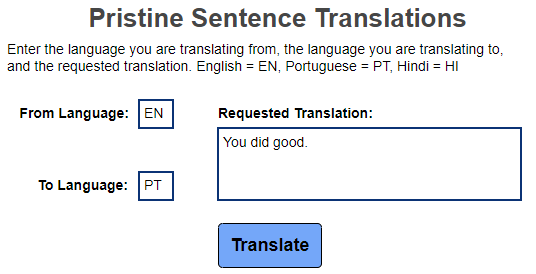
\includegraphics[width=.9\textwidth]{Screen_top.png}}
			\captionof{figure}{Language Input}
			\label{fig:Language Input}
		\end{center}
	\end{minipage}

After the user has entered the data and hit the ``Translate'' button the information is passed to our python text-processing. First our model finds the closest linguistic match to the sentence entered to a sentence for which the translation is known. Then we have a separate post-processing step to calculate how close of a match the input sentence is to the matched sentence, and we retrieve that translations of that sentence for the requested language. See Figure 1 in Section 4 for a visual reference.
The results are then returned to the screen for display. Note that there can be more than one valid translation for an input sentence, provided our database has the mappings:

	\begin{minipage}{\linewidth}
		\begin{center}
  			 \noindent\makebox[\textwidth]{%
			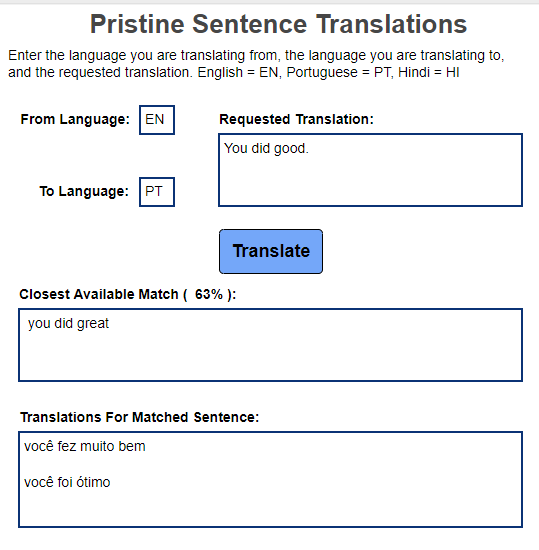
\includegraphics[width=.9\textwidth]{Screen.png}}
			\captionof{figure}{Display Translations}
			\label{fig:Display Translations}
			\vspace*{1cm}
		\end{center}
	\end{minipage}

If the user wants to try another sentence the user can change any of the three inputs above and hit the ``Translate'' button again to repeat the process.

	\section{Results and Analysis}
	After we assembled our database of translations and built our PKL files our only outstanding task was to pick a method for determining how close sentences are. We had two contenders: Euclidean Distances and Cosine Similarities. We needed a way to determine, given our dataset, which method stood the best chance of matching an input sentence to the sentence we thought it should match to. We decided to try slightly altering some of our pristine sentences in our database and running them through both comparisons, then analyze how well each method performed.

	To start, we altered our known sentence ``'we are good friends'' to ``we are best friends'', and ran it through the Euclidean Distance and Cosine Similarity comparisons. For the full code please reference \hyperlink{Appendix C}{Appendix C}.

	\begin{table} 
		\begin{center}
			\begin{tabular}{| l | l | l | l |}
			  \hline			
			  Method & Resulting Text & Distance/\% Match & Top 2 \% Diff \\
			  \hline			
			  Euclidean Distance & we are good friends & 72.18 & 62.31 \\
			  \hline			
			  Cosine Similarity & we are good friends & 73.95 & 135.73 \\
			  \hline  
			  Siamese LSTM & we are good friends & 75.22 & 73.8 \\
			  \hline
			\end{tabular}
		\end{center}
		\captionof{table}{``We Are Best Friends'' Match Test}
		\label{table:``We Are Best Friends'' Match Test}
	\end{table}

	All three methods were effective at finding the result we anticipated: ``We are good friends.'' However, examining the second-best guess score in each comparison shows that the cosine similarity method seemed much better at finding that result. The next-closest for Siamese MaLSTM was 73.8\%, Euclidean Distance was only 62.31\% more than the best guess, but for Cosine Similarity the best guess was 135.73\% better than the next-best guess. Even though all performed admirably in this circumstance, it seems like cosine similarity was able to more clearly differentiate the sentence we want from the sentence we don't.  To demonstrate the end-to-end process, in \hyperlink{Appendix D}{Appendix D} we show that our pristine sentence result of ``we are best friends'' translates to the Portuguese sentence ``Nós somos bons amigos''.

	We tried many examples and the results were similar, here is another example where we altered our known sentence ``I would like dessert'' to ``I would love dessert'', the code example can be found in \hyperlink{Appendix E}{Appendix E} :


	\begin{table} 
		\begin{center}
			\begin{tabular}{| l | l | l | l |}
			  \hline			
			  Method & Resulting Text & Distance/\% Match & Top 2 \% Diff \\
			  \hline			
			  Euclidean Distance & I would like dessert & 77.26 & 46.48 \\
			  \hline			
			  Cosine Similarity & I would like dessert & 70.16 & 95.07 \\
			  \hline  
			  Siamese LSTM & I would like dessert & 60.94 & 52.72 \\
			  \hline
			\end{tabular}
		\end{center}
		\captionof{table}{``I Would Love Dessert'' Match Test}
		\label{table:``I Would Love Dessert'' Test}
	\end{table}



	Again, both methods were effective at finding the result we anticipated: ``I would like dessert.'' However, the next-closest Euclidean Distance was only 46.48\% more than the best guess,  the next-closest Siamese similarity was 52.72\% more than the best guess, but for Cosine Similarity the best guess was 95.07\% better than the next-best guess. 

	We also thought that it would be interesting to try a sentence that wasn't close to one for which we knew the translation. For this we altered ``I would like some water'' to ``I would like some blueberry muffins and orange juice, please.''  \hyperlink{Appendix F}{Appendix F} has the code example, here is the result:



	\begin{table} 
		\begin{center}
			\begin{tabular}{| l | l | l | l |}
			  \hline			
			  Method & Resulting Text & Distance/\% Match & Top 2 \% Diff \\
			  \hline			
			  Euclidean Distance & I would like some water & 113.03 & 0.82 \\
			  \hline			
			  Cosine Similarity & I would like some water & 36.12 & 3.01 \\
			  \hline  
			  Siamese LSTM & I would like some water & 25.66 & 7.02 \\
			  \hline
			\end{tabular}
		\end{center}
		\captionof{table}{``I Would Like Some Blueberry Muffins and Orange Juice, Please'' Match Test}
		\label{table:``I Would Like Some Blueberry Muffins and Orange Juice, Please'' Test}
	\end{table}


	All three methods found what we hoped: ``I would like some water.'' Cosine Similarity did perform very slightly better than Euclidean Distance in terms of the difference to the next-highest match: 3.01\% for Cosine Similarity vs. 0.82\% for Euclidean Distance, but Siamese Similarity handled this difficult problem with the most distinction, with a distance of 7.02\% between the top and second-best guess. However, looking at the quality of match for Cosine Similarity says that these sentences are only 36.12\% similar and the Siamese Similarity is only 25.66\% similar, which are very low similarity scores compared to the over 60\% of the other two matches. This low score serves as a caution to the user to discourage anyone from taking this translation as a close match to what is entered.

	Finally, we wanted to list the point of PST, translating a sentence that is hard to translation from one language to another. In this case we chose ``You really hit one out of the park''. Google Translate shows this in Portuguese as ``Você realmente bateu um fora do Parque'', which still would not give a native Portuguese speaker any idea what that sentence means to them, unless they knew American Baseball. Here's how PST Performs, \hyperlink{Appendix G}{Appendix G} has the code:




	\begin{table} 
		\begin{center}
			\begin{tabular}{| l | l | l | l |}
			  \hline			
			  Method & Resulting Text & Distance/\% Match & Top 2 \% Diff \\
			  \hline			
			  Euclidean Distance & you hit one out of the park & 41.99 & 191.66 \\
			  \hline			
			  Cosine Similarity & you hit one out of the park & 91.18 & 264.79 \\
			  \hline  
			  Siamese LSTM & you hit one out of the park & 75.08 & 108.14 \\
			  \hline
			\end{tabular}
		\end{center}
		\captionof{table}{``You Really Hit One Out of the Park'' Match Test}
		\label{table:``You Really Hit One Out of the Park'' Test}
	\end{table}

	The sentence we input was very similar to the PST entry ``You hit one out of the park'', which is reflected in the displayed scores. More importantly, PST returned ``Você foi ótimo'', which means ``You were great'' in English, which is the intent of the colloquialism. 

	For another example, in Portuguese there's a popular sentence ``Eu adoro Cafuné''. Google Translate does not have a translation for ``Cafuné'', a complicated word which loosely means ``the act of running fingers through hair''. PST returns an English translation ``I love the feeling of fingers running through my hair'' when asked to translate ``Eu adoro Cafuné'' from Portuguese into English. Translating from sentence to sentence provides us a method to translate any sentence or concept into another language given enough time and resources.

	Now that we have performed our analysis we are ready to decide on a final method. All of code for our comparisons can be found at this URL in the References section: ~\cite{ref_url20}
	
	\subsection{Results and Analysis}
	Cosine Similarity consistently outperformed Euclidean Distance as a determination of sentence similarity, so that is the metric we will focus on for determining closeness of input sentences to our known sentences. It makes sense that Cosine Similarity would be a more ideal fit than Euclidean Sentences because every unexpected word in Euclidean Distance comparison is penalized, but in Cosine Similarity these are ignored, and we focus only on the matches. This helps cut through the noise and return a more confident match in what we want. 
	Cosine Similarity vs. Siamese Similarity is a much closer match. While Cosine Similarity, in general, had a higher percentage match and a larger distance between the top two matches, there two key factors to remember. The Siamese translation was pulling from a much larger dataset, over 400,000 records compared to only 200. This means the difference between the first and second guess could be understandably lower, since there is likely a closer sentence in the 400,000 sentences. Also, in our sentence with the most differences, Siamese Similarity had a wider margin than cosine similarity. For this reason, we will select Siamese Similarity as our preferred similarity metric.

	In addition, by testing a very bad sentence match we touched on the possibility of using a similarity threshold of some kind, where perhaps in future iterations of the program we could warn users not to pay too much attention to a sentence match less than some percentage. A match with at least 60\% similarity seems like a good match, below 40\% seems like a bad match, but we need to compare more data to determine what that threshold might make sense to be.

	We have also shown how PST could be used to overcome some of the hazards around language translation today, ignoring colloquialisms and focusing on the intent of the sentence.

	Given our work so far, we now have a method to find a sentence ID that is our closest match to an input sentence, then take that sentence ID and find all the applicable known translations for that sentence. We can do this for all 200 sentences in our database, and can display how close of a match we have made using Cosine Similarity, which we have identified as our chosen similarity determination method. This is enough to demonstrate the basic concept of PST, and can be expanded on for future work.

	\section{Ethical Considerations}
	Ethical considerations help outline the moral principles, principles about what is good or bad, that come into effect for a topic. In order to determine if we were meeting our moral obligations with this work we asked ourselves who will be affected by our work, and how we can ensure we are doing good to that group without harming another group. To answer the first question: the people affected by our work will be the users of our translation program, and the people with whom they speak. To answer the second question: we can ensure our translation process is as clear as possible, and we can provide the user with enough information to make an informed decision around his or her communication. 

	How can we be sure that our data we are providing to the user will be helpful instead of harmful? For example, if we provide a bad translation to a user then a well-meaning user could end up saying something inappropriate to a stranger or coworker, leading to negative repercussions such as exclusion, or disciplinary actions. In order to find a framework in which to address this ethical consideration, we found it helpful to have a template with some core questions to answer. Margot Mieske proposes in her paper ``A Quantitative Study of Data in the NLP community'' five key questions every NLP programmer must answer: ~\cite{ref_url8}


	\begin{table} 
		\begin{center}
			\begin{itemize}
				\item Has data been collected? 
				\item How was this data collected and processed? 
			 	\item Was previously available data used/extended – which one? 
				\item Is a link or a contact given? 
				\item Where does it point (private page, research institute, official repository)?
			\end{itemize}
		\end{center}
		\captionof{table}{Ethical Questions}
		\label{List: Ethical Questions}
	\end{table}

We answer each of these questions in turn. First, yes, data was collected for this project. For this project the initial set of 200 English Sentences data were gathered from three travel websites. Second, yes, we processed the data using removal of several characters as detailed in the Data section. Third, we extended this data using a couple of test sentences of our own, shown in in Table 5 in the Results and Analysis section. We did this to explore some popular colloquialisms and explore our problem statement. To answer the fourth and fifth questions together, the links for the travel sites are public URLs detailed here: ~\cite{ref_url11,ref_url12,ref_url13}. Travel sites were chosen in order to get a good spread of what sentences people might find useful. We also met with native speakers of our languages and had them review the translations to make sure the translations provided by the travel sites made sense. 

If there were gaps in the translations provided by the travel sites, we used a combination of Google Translate~\cite{ref_url14} and human expertise in Portuguese and German in order to determine if the Google Translation made sense. If the sentence did not make sense as Google Translated it, we entered a more sensible translation from human expertise. The original list of sentences and translations can be found in our public GitHub Repository here:
\url{https://github.com/coarib/SMU_Masters_PST/blob/master/data/processed/PST_workbook.xlsx}

For the specifics around ethical considerations for NLP we turn to Jochen L. Leidner and Vassilis Plachouras and their paper ``Ethical by Design: Ethics Best Practices for Natural Language Processing''~\cite{ref_url15}.  Leidner and Plachouras propose that since NLP pertains to human language and touches every part of human life it has a specific ethics dimension, therefore automation and errors also become ethical topics. We need to make sure our translations and base sentences are unbiased and fair, without discrimination based on age, race, or gender. This is why we chose to target travel sites that hopefully won't favor certain demographics. At the very least we are transparent about from where we pulled the sentences.

We carefully scanned each translation for fairness to make sure our data was reviewed before putting it out to the public, and we keep a tight control over the sentences that might be suggested for a user. With PST using curators to craft the translation by hand there is an increased potential for a curator to use bad translations in order to purposefully mislead a user. We had the translations peer-reviewed to mitigate this risk, and will need to continue this for the lifetime of the program.

This proof-of-concept system is not something we recommend putting into the world for general use. With only 200 sentences the risks around mistranslating something are too high, there is the potential for widespread confusion if our suggestions aren't close enough to the input request. That confusion has the potential to do harm to others, violating the ACM Code of Ethics section "1.2 Avoid Harm". Before going public we would need to follow Leidner and Plachouras's advice and establish an ethics review board that establish a process for reviewing and implementing new translation requests and helping monitor issues around translations on the site. 
	
	\section{Conclusions}
	Through this proof-of-concept we concluded that by moving the granularity of translations up to the sentence level we can get closer to the idea behind a sentence, and that enables us to translate colloquialisms, idioms, and slang between languages. We have given examples of deep learning models using the Keras API that returns close matches to sentences, and have identified Siamese Similarity as our preferred method of sentence comparisons, its matrix-based approach to sentence comparisons seemed to be the most resilient to a variety of sentence structures. We discovered that a match of over 60\% similarity was visually close to the sentence that was input and therefore would be most useful to a user attempting to find a viable translation for a sentence. We also concluded that our sentence matches were insufficient to be a global solution at this time, as our closeness metrics were often very low, and that more pristine sentence matches would help improve our models and the usefulness of PST.

\begin{thebibliography}{8}
	
	
\bibitem{ref_url1}
	\sloppy
	Google’s new translation software is powered by brainlike artificial intelligence (2016, September 27), Available at:

	\url{https://www.sciencemag.org/news/2016/09/google-s-new-translation-software-powered-brainlike-artificial-intelligence?r3f\_986=https://www.google.com/}.  Last accessed 4 Feb 2019
	
	
\bibitem{ref_url2}
	Found in translation: More accurate, fluent sentences in Google Translate (2016, November 15), Available at: \url{https://www.blog.google/products/translate/found-translation-more-accurate-fluent-sentences-google-translate}.  Last accessed 4 Feb 2019

\bibitem{ref_url3}
	A ten-minute introduction to sequence-to-sequence learning in Keras, Available at: \url{https://blog.keras.io/a-ten-minute-introduction-to-sequence-to-sequence-learning-in-keras.html}.  Last accessed 4 Feb 2019

\bibitem{ref_url4}
	Tab-delimited bilingual sentence pairs \url{http://www.manythings.org/anki/}.Last accessed  10 July 2019
		
\bibitem{ref_url6}
	Figure 3. Available at: \url{https://cdn-images-1.medium.com/max/1600/1*SQAxk6gSUM_AK2d53neYmA.jpeg}. Last accessed 22 Mar 2019

\bibitem{ref_url7}
	Figure 4, Available at: \url{https://s3-ap-south-1.amazonaws.com/av-blog-media/wp-content/uploads/2019/01/architecture.png}. Last accessd 22 Mar 2019
	
\bibitem{ref_url8}
	A Quantitative Study of Data in the NLP community, Margot Mieskes, Available at: \url{http://www.ethicsinnlp.org/workshop/EthNLP-2017.pdf}.  Last accessed 25 Mar 2019

\bibitem{ref_url10}
	Found in translation: More accurate, fluent sentences in Google Translate (2016, November 15), Available at: \url{https://www.blog.google/products/translate/found-translation-more-accurate-fluent-sentences-google-translate}.  Last accessed 25 Mar 2019

\bibitem{ref_url11}
	76 English Phrases for Traveling with Ease, Available at: \url{https://www.fluentu.com/blog/english/english-travel-phrases/}.  Last accessed 25 Mar 2019

\bibitem{ref_url12}
	Travel English-- 100 sentences you must know, Available at: \url{https://www.rong-chang.com/travel/}.  Last accessed 25 Mar 2019

\bibitem{ref_url13}
	100 Common English Phrases and Sentence Patterns (With Dialogue), Available at: \url{https://basicenglishspeaking.com/100-common-phrases-and-sentence-patterns/}.  Last accessed 25 Mar 2019

\bibitem{ref_url14}
	Google Translate, Available at: \url{https://translate.google.com/}.  Last accessed 25 Mar 2019

\bibitem{ref_url15}
	Ethical by Design: Ethics Best Practices for Natural Language Processing, Jochen L. Leidner and Vassilis Plachouras, Available at: \url{http://www.ethicsinnlp.org/workshop/pdf/EthNLP02.pdf/}.  Last accessed 25 Mar 2019

\bibitem{ref_url16}
Sequence to Sequence Learning with Neural Networks, Available at: \url{https://papers.nips.cc/paper/5346-sequence-to-sequence-learning-with-neural-networks.pdf/}.  Last accessed 25 Mar 2019

\bibitem{ref_url17}
SQL Alchemy, Available at: \url{https://www.sqlalchemy.org/}.  Last accessed 25 Mar 2019

\bibitem{ref_url18}
Found in translation: More accurate, fluent sentences in Google Translat, by Catherine Matacic on Sep. 27, 2016,  Available at:  \url{https://www.sciencemag.org/news/2016/09/google-s-new-translation-software-powered-brainlike-artificial-intelligence?r3f 986=https://www.google.com/}.  Last accessed 25 Mar 2019

\bibitem{ref_url19}
What is Euclidean Distance?, On April 1, 2017, Available at:  \url{What is Euclidean Distance?  https://machinelearningtutorials.com/euclidean-distance/}.  Last accessed 25 Mar 2019

\bibitem{ref_url20}
Text Similarities, Meenu Ahluwalia and Brian Coari, Available at:  \url{https://github.com/coarib/SMU_Masters_PST/blob/master/src/TextSimilarity_edited.ipynb}.  Last accessed 25 Mar 2019

\bibitem{ref_book1}
Jiawei Han, Micheline Kamber and Jian Pei: Data Mining: Concepts and Techniques. 3rd ed. Elsevier Inc., Chapter 2.4.7 - Cosine Similarity, Page 77 (2012)

\bibitem{ref_url21}
Siamese Recurrent Architectures for Learning Sentence Similarity (2016), Available at:
\url{https://www.aaai.org/ocs/index.php/AAAI/AAAI16/paper/view/12195/}.

\bibitem{ref_url23}
Google's word2ve,c Available at:
\url{https://code.google.com/archive/p/word2vec//}.

\bibitem{ref_url24}
Siamese Recurrent Architectures for Learning Sentence Similarity, Available at:
\url{http://people.csail.mit.edu/jonasmueller/info/MuellerThyagarajan_AAAI16.pdf/}.

\bibitem{ref_url25}
Kaggle Quora Question Pairs  Dataset, Available at: 
\url{https://www.kaggle.com/c/quora-question-pairs/}.

\bibitem{ref_url26}
Infornation Retrieval, Available at: 
\url{https://nlp.stanford.edu/IR-book/pdf/irbookonlinereading.pdf/}.

\end{thebibliography}


\appendix

\section{GitHub Repository}
	\url{https://github.com/coarib/SMU_Masters_PST/blob/master/data/processed/PST_workbook.xlsx}

\section{SQL Queries}
Select the text and sentence IDs for a language key. Language keys can be EN, PT, or DE for English, Portuguese, or German, respectively. 

\begin{verbatim}
select text, sentence_id from Sentences where language_key='[Language_Key]'
\end{verbatim}
Select every combination of matching translations between all sentences. Storing this query in a dataframe allows us to get all the translations for a sentence just by matching a sentence ID to the input\_sentence\_id column.

\begin{verbatim}
SELECT a.sentence_id as input_sentence_id, 
a.language_key as input_language_key, a.text as input_text, 
b.text as output_text, b.sentence_id as output_sentence_id, 
b.language_key as output_language_key FROM masters.Translations 
left join masters.Sentences a on a.sentence_id=Translations.sentence_id_1 
left join masters.Sentences b on b.sentence_id=Translations.sentence_id_2
\end{verbatim}

\section{Cosine Similarity and Euclidean Distance Comparison}
\hypertarget{Appendix C}{}


	\begin{minipage}{\linewidth}
		\begin{center}
			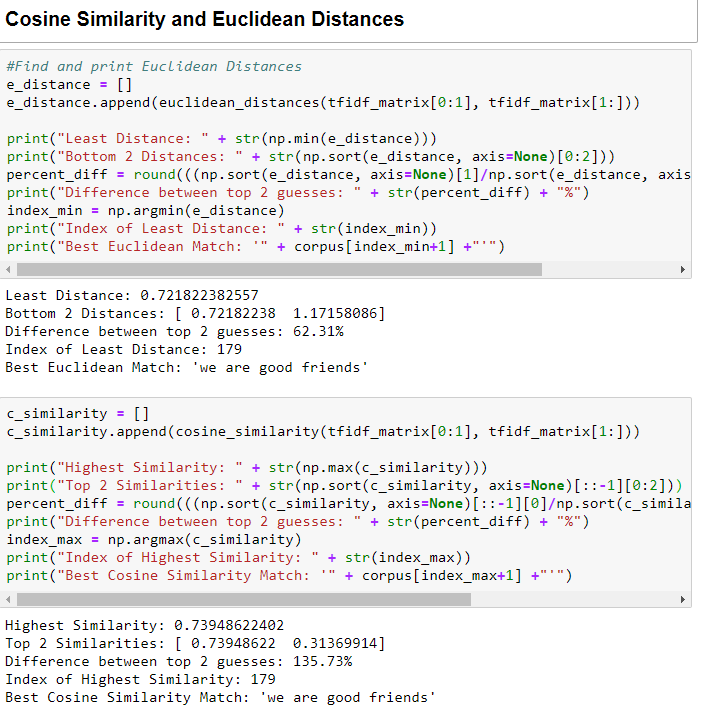
\includegraphics[width=\linewidth]{Friends_Comparison.png}
			\captionof{figure}{Sentence Comparison 1}
			\label{fig:Sentence Comparison 1}
			\vspace*{1cm}
		\end{center}
	\end{minipage}
	\afterpage{\clearpage}


\section{``we are best friends'' Translation Example}
\hypertarget{Appendix D}{}


	\begin{minipage}{\linewidth}
		\begin{center}
			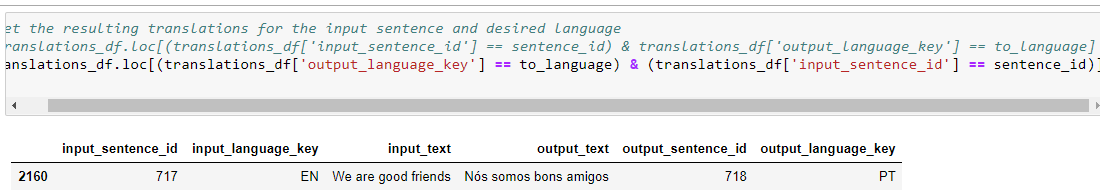
\includegraphics[width=\linewidth]{Language_Match.png}
			\captionof{figure}{Translating Matched Sentence to Portuguese}
			\label{fig:Translating Matched Sentence  to Portuguese}
			\vspace*{1cm}
		\end{center}
	\end{minipage}
	\afterpage{\clearpage}



\section{``I would love dessert'' Translation Example}
\hypertarget{Appendix E}{}

	\begin{minipage}{\linewidth}
		\begin{center}
			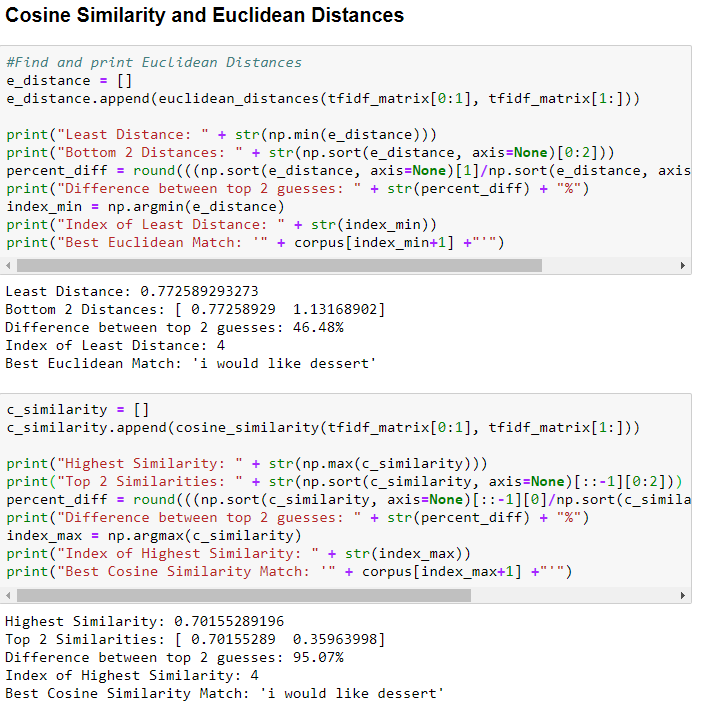
\includegraphics[width=\linewidth]{Dessert_Comparison.png}
			\captionof{figure}{Sentence Comparison 2}
			\label{fig:Sentence Comparison 2}
			\vspace*{1cm}
		\end{center}
	\end{minipage}
	\afterpage{\clearpage}


\section{``I would like some blueberry muffins and orange juice, please.'' Translation Example}
\hypertarget{Appendix F}{}

	\begin{minipage}{\linewidth}
		\begin{center}
			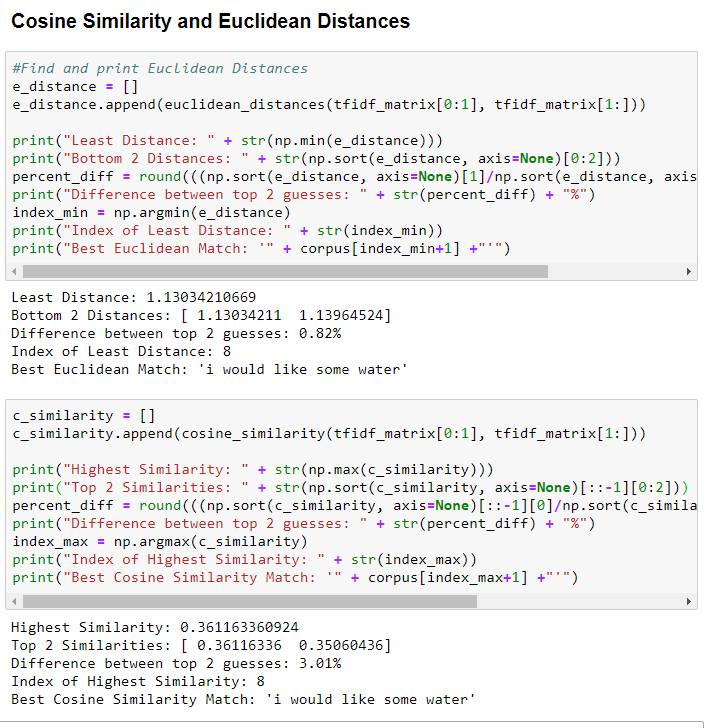
\includegraphics[width=\linewidth]{Terrible_Comparison.png}
			\captionof{figure}{Sentence Comparison 3}
			\label{fig:Sentence Comparison 3}
			\vspace*{1cm}
		\end{center}
	\end{minipage}
	\afterpage{\clearpage}

\section{``You really hit one out of the park.'' Translation Example}
\hypertarget{Appendix G}{}
	\begin{minipage}{\linewidth}
		\begin{center}
			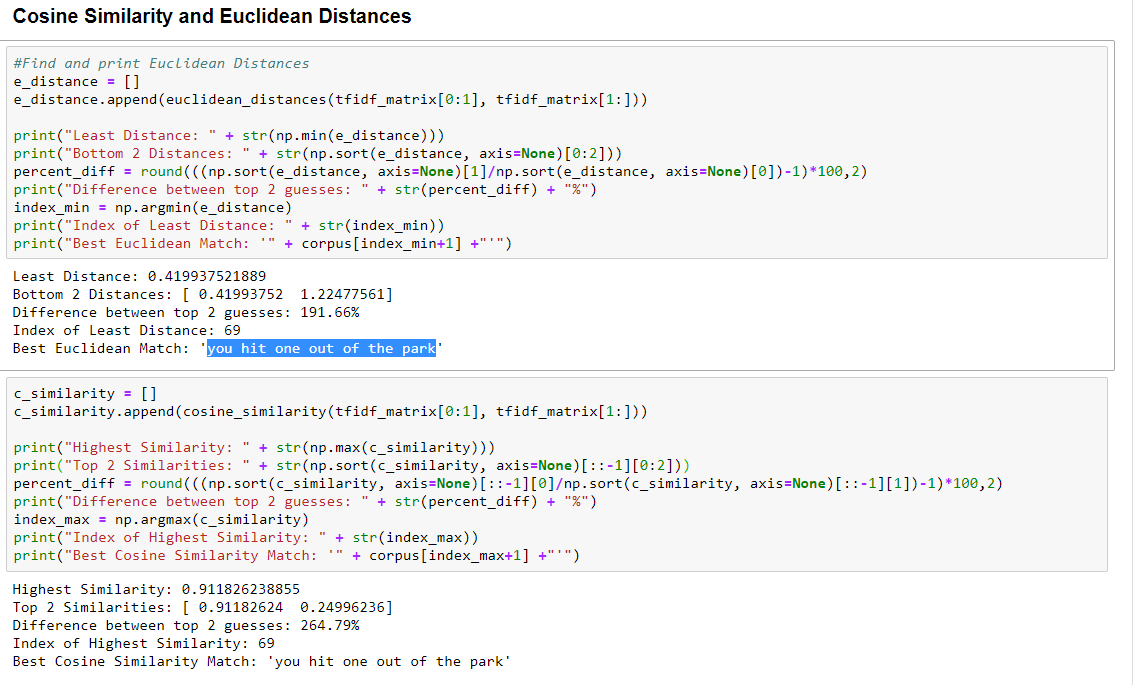
\includegraphics[width=\linewidth]{Park_Comparison.png}
			\captionof{figure}{Sentence Comparison 4}
			\label{fig:Sentence Comparison 4}
			\vspace*{1cm}
		\end{center}
	\end{minipage}
	\afterpage{\clearpage}
	\begin{minipage}{\linewidth}
		\begin{center}
			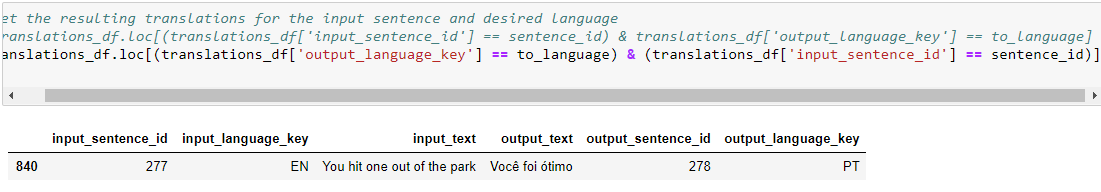
\includegraphics[width=\linewidth]{Park_Translation.png}
			\captionof{figure}{Translation for Colloquialism}
			\label{fig:Translation for Colloquialism}
			\vspace*{1cm}
		\end{center}
	\end{minipage}
	\afterpage{\clearpage}
\end{document}